\documentclass{Z}
%% need no \usepackage{Sweave}


\title{HCL-based Color Palettes in \proglang{R}}
\Plaintitle{HCL-based Color Palettes in R}
\author{Achim Zeileis \textnormal{and} Kurt Hornik\\Wirtschaftsuniversit\"at Wien, Austria}
\Plainauthor{Achim Zeileis, Kurt Hornik}
\Keywords{HCL colors, qualitative palette, sequential palette, diverging palette}

\Abstract{
  The package \pkg{vcd} provides various functions providing perceptually-based
  color palettes for coding categorical data (qualitative palettes) and numerical
  variables (sequential and diverging palettes). We illustrate how these
  functions can be employed to generate various flavours of these palettes (with
  different emphases) and how they can be plugged into \proglang{R} graphics
  functions.
}

\begin{document}

%\VignetteIndexEntry{HCL-based Color Palettes in R}
%\VignetteDepends{vcd,colorspace,MASS,KernSmooth,mvtnorm,kernlab}
%\VignetteKeywords{HCL colors, qualitative palette, sequential palette, diverging palette}
%\VignettePackage{vcd}


\section{Introduction} \label{sec:intro}

This is a companion vignette to \cite{vcd:Zeileis+Hornik:2006} providing
further technical details on the construction of the palettes as well as
\proglang{R} code illustrating the use of varying palettes in practice.
The palettes as well as some graphical functions demonstrated are contained
in the package \pkg{vcd}.
As a simple convenience function we will use the function
\begin{Schunk}
\begin{Sinput}
> pal <- function(col, border = "light gray", ...) {
+     n <- length(col)
+     plot(0, 0, type = "n", xlim = c(0, 1), ylim = c(0, 1), axes = FALSE, 
+         xlab = "", ylab = "", ...)
+     rect(0:(n - 1)/n, 0, 1:n/n, 1, col = col, border = border)
+ }
\end{Sinput}
\end{Schunk}
which displays a set of colors using a sequence of shaded rectangles.

In the remainder of this vignette, we first outline how different types of palettes
can be constructed and generated using the tools from \pkg{vcd}. Subsequently,
we present a collection of examples illustrating the tools in practice.


\section{Color palettes} \label{sec:palettes}

\subsection{Qualitative palettes} \label{sec:qualitative}

Qualitative palettes are sets of colors for depicting different categories,
i.e., for coding a categorical variable. To give the same
perceptual weight to each category, chroma and luminance are kept 
and only the hue is varied for obtaining different colors
(which are consequently all balanced towards the same gray). 

In \pkg{vcd}, qualitative palettes are implemented in the function
\begin{Soutput}
rainbow_hcl(n, c = 50, l = 70, start = 0, end = 360*(n-1)/n, ...)
\end{Soutput}
where \code{n} controls the number of colors in the palette. The arguments
\code{c} and \code{l} give the fixed chroma and luminance levels, respectively,
and \code{start} and \code{end} specify the range of hue angles. The function
is named after the base \proglang{R} function \code{rainbow()} which has a similar
interface but chooses colors in HSV coordinates.
Figure~\ref{fig:pal-q-examples} depicts
examples for generating qualitative sets of colors $(H, 50, 70)$ produced by
\begin{Schunk}
\begin{Sinput}
> pal(rainbow_hcl(4, start = 30, end = 300), main = "dynamic")
> pal(rainbow_hcl(4, start = 60, end = 240), main = "harmonic")
> pal(rainbow_hcl(4, start = 270, end = 150), main = "cold")
> pal(rainbow_hcl(4, start = 90, end = -30), main = "warm")
\end{Sinput}
\end{Schunk}
From left to right and top to down, this shows a palette from the full spectrum ($H = 30, 120, 210, 300$)
creating a `dynamic' set of colors, a `harmonic'
set with $H = 60, 120, 180, 240$, warm colors (from the blue/green part of the spectrum: 
$H = 270, 230, 190, 150$) and cold colors (from the yellow/red part of the spectrum:
$H = 90, 50, 10, 330$), respectively.

\setkeys{Gin}{width=0.8\textwidth}
\begin{figure}[p]
\begin{center}
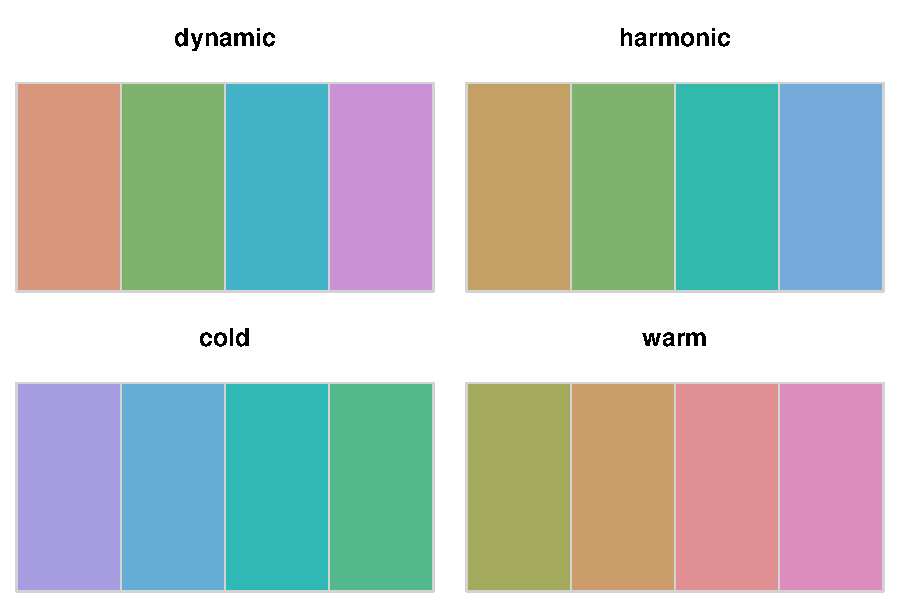
\includegraphics{hcl-colors-pal-q1}
\caption{\label{fig:pal-q-examples} Examples for qualitative palettes. Hue is varied
in different intervals for given $C = 50$ and $L = 70$.}
\end{center}
\end{figure}


\subsection{Sequential palettes} \label{sec:sequential}

Sequential palettes are used for coding numerical information that ranges
in a certain interval where low values are considered to be uninteresting and
high values are interesting. Suppose we need to visualize an intensity or
interestingness $i$ which (without loss of generality) is scaled to the unit
interval.

Potentially, all three dimensions of HCL space can be used for coding the intensity,
leading to colors from an interval of hues (i.e., differing types of colors),
an interval of chroma values (i.e., differing colorfulness) and an interval of
luminance (i.e., differing intensity of gray). If we allow chroma and luminance
to increase non-linearly via a function of type $i^p$, the resulting formula is:
  \[ (H_2 - i \cdot (H_1 - H_2), C_{\max} - i^{p_1} \cdot (C_{\max} - C_{\min}),
      L_{\max} - i^{p_2} \cdot (L_{\max} - L_{\min})). \]

Two different ``flavors'' of this formula are readily implemented in \pkg{vcd},
employing different defaults. For single hue palettes with $H_1 = H_2$ the 
function
\begin{Soutput}
sequential_hcl(n, h = 260, c = c(80, 0), l = c(30, 90), power = 1.5, ...) 
\end{Soutput}
is provided where the first element of \code{c} and \code{l} give the starting chroma and luminance
coordinate (by default colorful and dark) and the second element the ending coordinate
(by default light gray). The \code{power} argument implements the parameter $p$ 
from the $i^p$ function (and can be a vector of length 2). Sequential palettes using an
interval of hues are provided by
\begin{Soutput}
heat_hcl(n, h = c(0, 90), c = c(100, 30), l = c(50, 90), power = c(1/5, 1), ...)
\end{Soutput}
named after the HSV-based \proglang{R} function \code{heat.colors()} and
by default starts from a red and going to a yellow hue. The defaults in \code{heat_hcl()}
are set differently compared to \code{sequential_hcl()} as to make the default HCL heat
colors more similar to the HSV version. The defaults of \code{sequential_hcl()}, on the
other hand, are set as to achieve a large contrast on the luminance axis. In addition
\code{terrain_hcl()} is a wrapper for \code{heat_hcl()} producing colors similar to
the HSV-based \code{terrain.colors()} from base \proglang{R}.

Various palettes produced from these functions are shown in
Figure~\ref{fig:pal-s-examples} using different pairs of hues as well as different
chroma and luminance contrasts.
\begin{Schunk}
\begin{Sinput}
> pal(sequential_hcl(12, c = 0, power = 2.2))
> pal(sequential_hcl(12, power = 2.2))
> pal(heat_hcl(12, c = c(80, 30), l = c(30, 90), power = c(1/5, 
+     2)))
> pal(terrain_hcl(12, c = c(65, 0), l = c(45, 90), power = c(1/2, 
+     1.5)))
> pal(rev(heat_hcl(12, h = c(0, -100), l = c(75, 40), c = c(40, 
+     80), power = 1)))
\end{Sinput}
\end{Schunk}

\setkeys{Gin}{width=.8\textwidth}
\begin{figure}[p]
\begin{center}
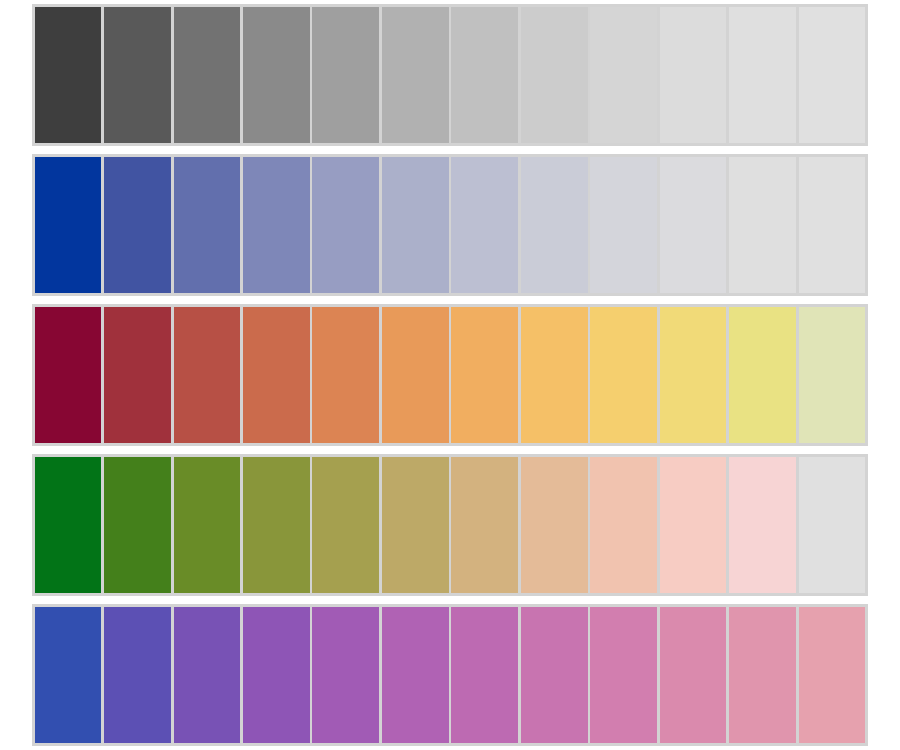
\includegraphics{hcl-colors-pal-s1}
\caption{\label{fig:pal-s-examples} Examples for sequential palettes, varying
only luminance (first panel), chroma and luminance (second panel), and hue,
chroma and luminance (remaining panels).}
\end{center}
\end{figure}


\subsection{Diverging palettes} \label{sec:diverging}

Diverging palettes are also used for coding numerical information ranging in a certain
interval---however, this interval includes a neutral value. Analogously to the previous
section, we suppose that we want to visualize an intensity or interestingness $i$
from the interval $[-1, 1]$ (without loss of generality).
Given useful sequential palettes, deriving diverging palettes is easy: two different hues are
chosen for adding color to the same amount of `gray' at a given intensity $|i|$.

Diverging palettes are implemented in the function
\begin{Soutput}
diverge_hcl(n, h = c(260, 0), c = 80, l = c(30, 90), power = 1.5, ...) 
\end{Soutput}
which has the same arguments as \code{sequential_hcl()} but takes a pair of hues \code{h}.

Figure~\ref{fig:pal-d-examples} shows various examples of conceivable combinations of
hue, chroma and luminance. The first palette uses a broader range on the luminance axis
whereas the others mostly rely on chroma contrasts.
\begin{Schunk}
\begin{Sinput}
> pal(diverge_hcl(7))
> pal(diverge_hcl(7, c = 100, l = c(50, 90), power = 1))
> pal(diverge_hcl(7, h = c(130, 43), c = 100, l = c(70, 90)))
> pal(diverge_hcl(7, h = c(180, 330), c = 59, l = c(75, 95)))
\end{Sinput}
\end{Schunk}

\setkeys{Gin}{width=.8\textwidth}
\begin{figure}[t!]
\begin{center}
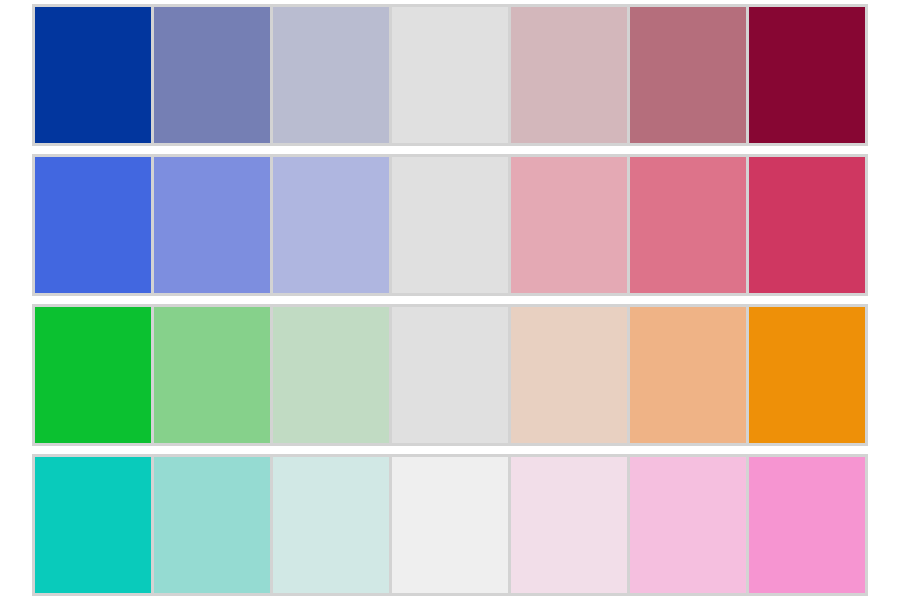
\includegraphics{hcl-colors-pal-d1}
\caption{\label{fig:pal-d-examples} Examples for diverging palettes with different
pairs of hues and decreasing luminance contrasts.}
\end{center}
\end{figure}

\section{Illustrations} \label{sec:illustrations}

\subsection{Qualitative palettes: Seats and votes in the German Bundestag}

In this section, we show a collection of examples for the various types of palettes applied
to statistical graphics. The first example illustrates qualitative palettes
and visualizes data from the 2005 election for the German parliament ``Bundestag''.
In this election, five parties were able to obtain enough votes to enter the
Bundestag, the numbers of seats are given by

\begin{Schunk}
\begin{Sinput}
> seats <- structure(c(226, 61, 54, 51, 222), .Names = c("CDU/CSU", 
+     "FDP", "Linke", "Gruene", "SPD"))
> seats
\end{Sinput}
\end{Schunk}

We choose colors that are rough metaphors for the political parties, using a red hue $H = 0$ for the
social democrats SPD, a blue hue $H = 240$ for the conservative CDU/CSU, a yellow hue $H = 60$
for the liberal FDP, a green hue $H = 120$ for the green party ``Die Gr\"unen'' and a purple 
hue $H = 300$ for the leftist party ``Die Linke''. To obtain rather intense colors, we set
chroma to $C = 60$ and luminance to $L = 75$:

\begin{Schunk}
\begin{Sinput}
> parties <- rainbow_hcl(6, c = 60, l = 75)[c(5, 2, 6, 3, 1)]
> names(parties) <- names(seats)
\end{Sinput}
\end{Schunk}

The distribution of seats is depicted in a pie chart in Figure~\ref{fig:seats}.
showing clearly that neither the governing
coalition of SPD and Gr\"une nor the opposition of CDU/CSU and FDP could assemble a majority.
Given that no party would enter a coalition with the leftists, this lead to a big coalition
of CDU/CSU and SPD. 
\begin{Schunk}
\begin{Sinput}
> pie(seats, clockwise = TRUE, col = parties, radius = 1)
\end{Sinput}
\end{Schunk}

\setkeys{Gin}{width=.6\textwidth}
\begin{figure}[p]
\begin{center}
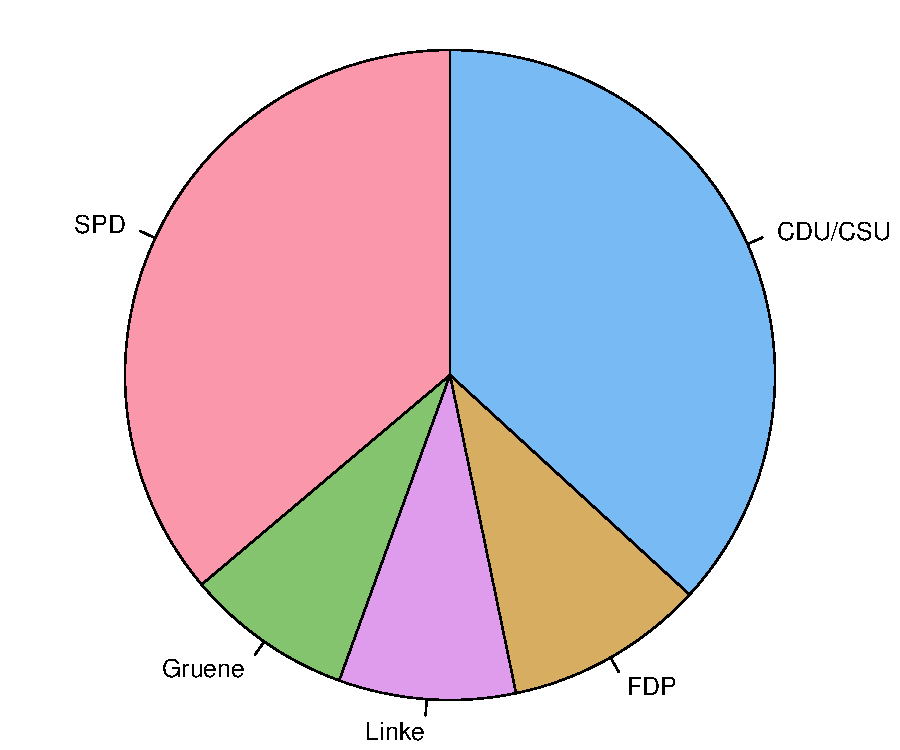
\includegraphics{hcl-colors-seats1}
\caption{\label{fig:seats} Seats in the German parliament.}
\end{center}
\end{figure}

To take a closer look at the regional distribution, we load the \code{Bundestag2005}
data set containing a contingency table with the number of votes for each party
stratified by province (Bundesland). Then, we re-order the provinces from 
north to south, first the 10 western provinces (the former Federal Republic of Germany, FRG),
then the 6 eastern provinces (the former German Democratic Republic, GDR). 
\begin{Schunk}
\begin{Sinput}
> data("Bundestag2005")
> votes <- Bundestag2005[c(1, 3:5, 9, 11, 13:16, 2, 6:8, 10, 12), 
+     c("CDU/CSU", "FDP", "SPD", "Gruene", "Linke")]
\end{Sinput}
\end{Schunk}

The data can then be visualized using a highlighted mosaic display via
\begin{Schunk}
\begin{Sinput}
> mosaic(votes, gp = gpar(fill = parties[colnames(votes)]))
\end{Sinput}
\end{Schunk}
The annotation for this plot is clearly sub-optimal, hence we use the 
flexible \code{strucplot()} framework provided by \pkg{vcd} and display
the data via
\begin{Schunk}
\begin{Sinput}
> mosaic(votes, gp = gpar(fill = parties[colnames(votes)]), spacing = spacing_highlighting, 
+     labeling = labeling_left, labeling_args = list(rot_labels = c(0, 
+         90, 0, 0), pos_labels = "center", just_labels = c("center", 
+         "center", "center", "right"), varnames = FALSE), margins = unit(c(2.5, 
+         1, 1, 12), "lines"), keep_aspect_ratio = FALSE)
\end{Sinput}
\end{Schunk}
The output is shown in Figure~\ref{fig:votes} highlighting that
the SPD performed better in the north and the CDU/CSU better in the south; furthermore,
Die Linke performed particularly well in the eastern provinces and in Saarland.


\setkeys{Gin}{width=.8\textwidth}
\begin{figure}[p]
\begin{center}
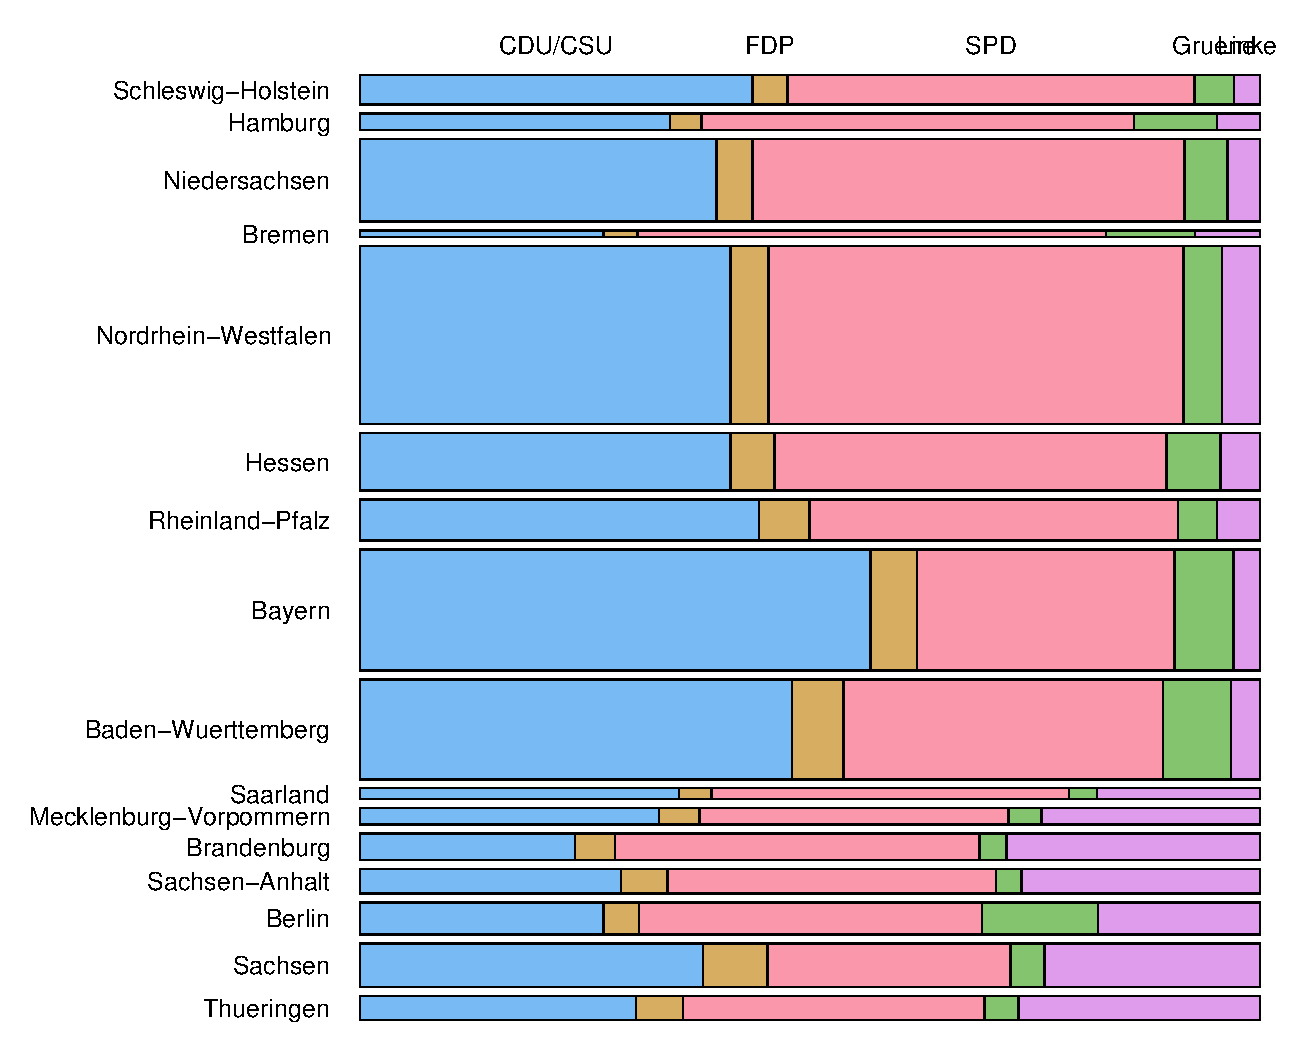
\includegraphics{hcl-colors-votes1}
\caption{\label{fig:votes} Votes in the German election 2005.}
\end{center}
\end{figure}

\subsection{Sequential palettes: Old Faithful geyser eruptions}

To illustrate sequential palettes, a bivariate density estimation for the Old
Faithful geyser eruptions data \code{geyser} from \pkg{MASS} is visualized.
The Old Faithful geyser is one of the most popular sites in Yellowstone National Park
and it is of some interest to understand the relation ship between the duration
of a geyser eruption and the waiting time for this eruption. To look at the data,
we use a bivariate kernel density estimate provided
by the function \code{bkde2D()} from package \pkg{KernSmooth}.
\begin{Schunk}
\begin{Sinput}
> library("KernSmooth")
> data("geyser", package = "MASS")
> dens <- bkde2D(geyser[, 2:1], bandwidth = c(0.2, 3), gridsize = c(201, 
+     201))
\end{Sinput}
\end{Schunk}

Subsequently, we look at the estimated kernel density by means of a heatmap
(produced via \code{image()}) using two different sequential palettes: first
with only gray colors
\begin{Schunk}
\begin{Sinput}
> image(dens$x1, dens$x2, dens$fhat, xlab = "duration", ylab = "waiting time", 
+     col = rev(sequential_hcl(33, c = 0, l = c(30, 90), power = c(1/5, 
+         1.5))))
\end{Sinput}
\end{Schunk}
and then using heat colors balanced towards the sam gray levels as above
\begin{Schunk}
\begin{Sinput}
> image(dens$x1, dens$x2, dens$fhat, xlab = "duration", ylab = "waiting time", 
+     col = rev(heat_hcl(33, c = c(80, 30), l = c(30, 90), power = c(1/5, 
+         1.5))))
\end{Sinput}
\end{Schunk}
Figure~\ref{fig:bkde} shows the resulting heatmaps revealing a multi-modal
bivariate distribution: short waiting
times (around 50 minutes) are typically followed by a long eruption (around 4 minutes)
whereas long waiting times (around 80 minutes) can be followed by either a long
or short eruption (around 4 minutes). 

\setkeys{Gin}{width=\textwidth}
\begin{figure}[t!]
\begin{center}
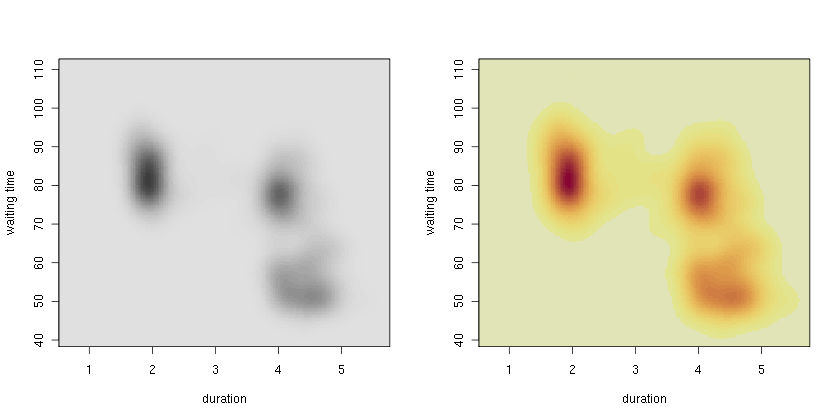
\includegraphics{bkde}
\caption{\label{fig:bkde} Bivariate density estimation for duration and waiting time for an eruption.}
\end{center}
\end{figure}

Another interesting question in this data set would be ask how long the waiting
time for the next eruption is following a short or long eruption respectively.
This can be visualized using another bivarate density estimate for the transformed
data set matching the previous duration with the following waiting time:
\begin{Schunk}
\begin{Sinput}
> library("KernSmooth")
> geyser2 <- cbind(geyser$duration[-299], geyser$waiting[-1])
> dens2 <- bkde2D(geyser2, bandwidth = c(0.2, 3), gridsize = c(201, 
+     201))
\end{Sinput}
\end{Schunk}

Again, we look at this density using two heatmaps generated via
\begin{Schunk}
\begin{Sinput}
> image(dens2$x1, dens2$x2, dens2$fhat, xlab = "duration", ylab = "waiting time", 
+     col = rev(sequential_hcl(33, c = 0, l = c(30, 90), power = c(1/5, 
+         1.5))))
\end{Sinput}
\end{Schunk}
and
\begin{Schunk}
\begin{Sinput}
> image(dens2$x1, dens2$x2, dens2$fhat, xlab = "duration", ylab = "waiting time", 
+     col = rev(heat_hcl(33, c = c(80, 30), l = c(30, 90), power = c(1/5, 
+         1.5))))
\end{Sinput}
\end{Schunk}
Figure~\ref{fig:bkde2} shows the result that illustrates that long and short
waiting times follow long and short eruption durations, resepectively.

\setkeys{Gin}{width=\textwidth}
\begin{figure}[t!]
\begin{center}
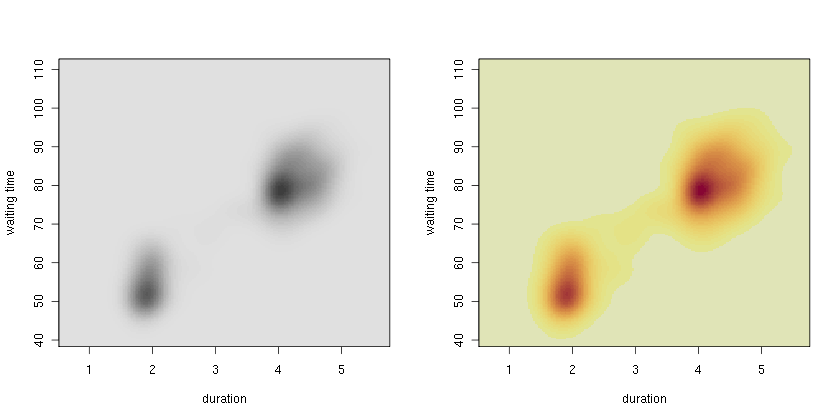
\includegraphics{bkde2}
\caption{\label{fig:bkde2} Bivariate density estimation for previous duration and following waiting time for
an eruption.}
\end{center}
\end{figure}

\subsection{Diverging palettes: Arthritis and SVM classification}

Diverging palettes are particularly useful
when visualizing residuals or correlations (with natural neutral value 0) or probabilities 
in 2-class supervised learning (with neutral value 0.5). Examples for both situations are
provided here. First, we look at the outcome for the female patients from a double-blind clinical
trial investigating a new treatment for rheumatoid arthritis. 
\begin{Schunk}
\begin{Sinput}
> art <- xtabs(~Treatment + Improved, data = Arthritis, subset = Sex == 
+     "Female")
\end{Sinput}
\end{Schunk}
For visualizing the data, we use a mosaic display with maximum shading
\citep[as derived by][]{vcd:Zeileis+Meyer+Hornik:2005} via
\begin{Schunk}
\begin{Sinput}
> set.seed(1071)
> mosaic(art, gp = shading_max, gp_args = list(n = 5000))
\end{Sinput}
\end{Schunk}

The mosaic rectangles in Figure~\ref{fig:arthritis} 
signal that the treatment lead to higher improvement compared to the placebo group; this effect
is shown to be significant by the shading that codes the size of the Pearon residuals.
Positive residuals, corresponding
to more observations in the corresponding cell than expected under independence, are depicted
in blue, negative residuals in red. Light colors signal significance at 10\% level, full colors
significance at 1\% level. The palette implicitly used in this plot is
\code{diverge_hcl(5, c = c(100, 0), l = c(50, 90), power = 1)}, it can be modified using
the arguments of \code{shading_max()} which has an interface similar to \code{diverge_hcl()}.

\setkeys{Gin}{width=.7\textwidth}
\begin{figure}[p]
\begin{center}
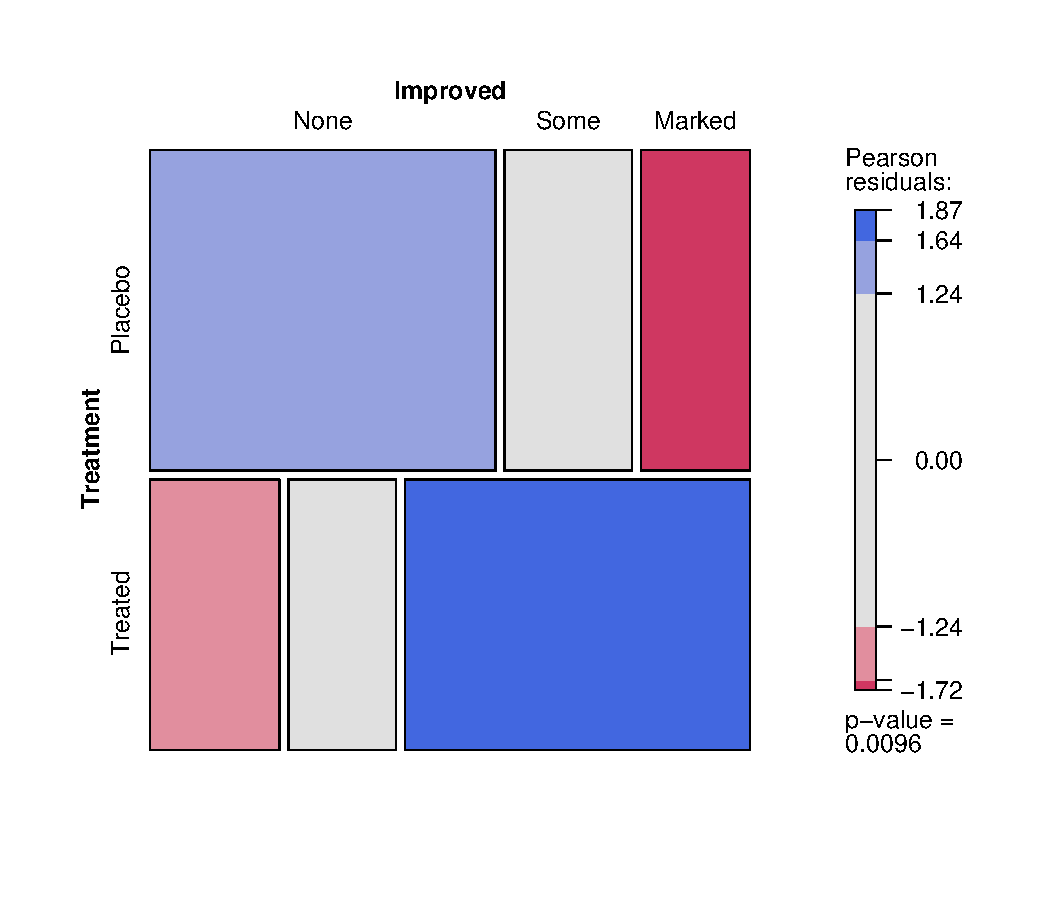
\includegraphics{hcl-colors-arthritis1}
\caption{\label{fig:arthritis} Extended mosaic display for arthritis data.}
\end{center}
\end{figure}

To illustrate the use of diverging palettes in 2-class classification, we generate
some artificial date from a mixture of two bivariate normal distributions with
different means and covariance matrices. The data are generated using \pkg{mvtnorm}
and collected in a data frame \code{ex1}:
\begin{Schunk}
\begin{Sinput}
> library("mvtnorm")
> set.seed(123)
> x1 <- rmvnorm(75, mean = c(1.5, 1.5), sigma = matrix(c(1, 0.8, 
+     0.8, 1), ncol = 2))
> x2 <- rmvnorm(75, mean = c(-1, -1), sigma = matrix(c(1, -0.3, 
+     -0.3, 1), ncol = 2))
> X <- rbind(x1, x2)
> ex1 <- data.frame(class = factor(c(rep("a", 75), rep("b", 75))), 
+     x1 = X[, 1], x2 = X[, 2])
\end{Sinput}
\end{Schunk}
We fit a support vector machine (SVM) with a radial basis function kernel to this data
set, using the function \code{ksvm()} from \pkg{kernlab}
\begin{Schunk}
\begin{Sinput}
> library("kernlab")
> fm <- ksvm(class ~ ., data = ex1, C = 0.5)
\end{Sinput}
\end{Schunk}
which can subsequently be easily visualized via
\begin{Schunk}
\begin{Sinput}
> plot(fm, data = ex1)
\end{Sinput}
\end{Schunk}
The resulting plot in Figure~\ref{fig:class} shows a heatmap with the fit of 
the SVM. The circles and triangles show the original observations, solid symbols correspond to
the support vectors found. The shading underlying the plot visualizes the fitted decision
values: values around 0 are on the decision boundary and are shaded in light gray, while
regions that are firmly classified to one or the other class are shaded in full blue and
red respectively. The palette used by the \code{plot()} method for \code{ksvm} objects
cannot be easily modified---however, the colors employed are equivalent to
\code{diverge_hcl(n, c = c(100, 0), l = c(50, 90), power = 1.3)}.

\setkeys{Gin}{width=.7\textwidth}
\begin{figure}[p]
\begin{center}
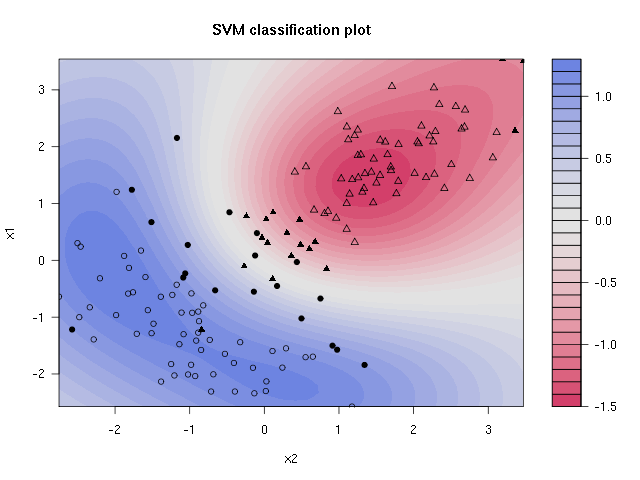
\includegraphics{class}
\caption{\label{fig:class} SVM classification plot.}
\end{center}
\end{figure}



\bibliography{vcd}

\end{document}
